
\documentclass[../skript.tex]{subfiles}

% Use standard labeling-order: 
%  		-	c 		chapter
% 		-	se 		section
% 		-	su 		subsection
% 		-	eq 		equation
% 		- 	fi 		figure
%
%

\chapter{Introduction}\label{c1}
	\section{Multiscale Problems}\label{c1se1}
		Applications include:
		\begin{itemize}
			\item Geophysical Flows in porous media
			\item Mechanical Simulation \& Design of composite materials
		\end{itemize}
		For further information about Multiscale Problems in general see \cite[Chapter 1]{lectureNotes}.

	\section{Modeling of diffusion in heterogeneous media}\label{c1se2}
		Imagine a motionless medium (or fluid) filling a straight and very thin tube, and a substance diffusion through it. What we have given is the concentration of the substance $u(t)$ at some time $t=0$, we are interested in the computation at later times.
		The amount of substance that passes the point $x$ from left to right is called flux $q(x,t)$. We assume conservation of mass, i.e.,
		for any control volume $(x_0,x_1)$, the mass 
		\begin{figure}[h]
			\centering
			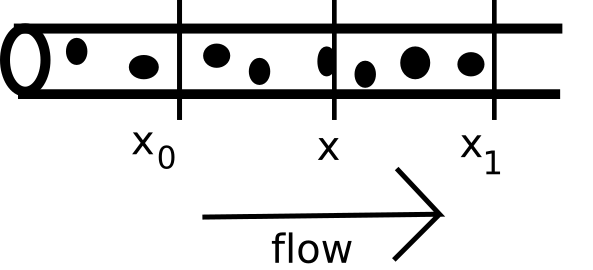
\includegraphics[width=0.25\textwidth]{Images/num1.png}
			\caption{Multiscale setting of a thin tube; shows the flux at the point $x$}
			\label{fig1}
		\end{figure}
		\[
			M = \int_{x_0}^{x_1} u(x,t)\,dx
		\]

		changes in time only by \emph{in-} or \emph{outflow}, i.e. the change of mass
		\[
			\frac{d}{dt} M = q(x_0,t) - q(x_1,t).
		\]
		The above equation states that the mass changes due to inflow at $x_0$ and outflow at $x_1$ at time $t$ (negative flow, i.e. outflow has negative sign).\par
		We rewrite this as 
		\[
			\int_{x_0}^{x_1}\frac{d}{dt} u(x,t)\,dx = q(x_0,t) - q(x_1,t).
		\]
		Differentiation w.r.t. $x_1$ and replacement of $x_1\mapsto x$ leads (assuming the standard interval in space)
		\[
			\frac{d}{dt}u = - \frac{d}{dx} q,\quad\text{in } Q = [0,1]\times[0,T].
		\]
		This conservation law does not determine $u$ and $q$. We need a second hypothesis that connects concentration and flux - a \emph{diffusion law} (experimental / phenomenological law). The simplest diffusion law is \textbf{Fick's first law} and says that the flux depends linearly on $u_x$
		\[
			q(x,t) = - A(x)\frac{d}{dx} u(x,t).
		\]
		The diffusivity $A(x) > 0$ is a characteristic property of the medium (material) at point $x$. In homogeneous media, $A$ may be treated as a global constant. In heterogeneous media, $A$ varies with spatial location (e.g. $A$ takes two different values in the fibers and in the background medium (\emph{matrix})). Finally, we model the process of diffusion by the linear PDE:
		\begin{equation}\label{c1se2eq1}
			\frac{d}{dt} u =\frac{d}{dx}\left(A\frac{d}{dx}u\right)\quad\text{in } Q
		\end{equation}
		along with the initial condition $u(x,0) = u_0(x)$, with $u_0$ denoting the given concentration at time $t=0$. If we want to model that no substance can enter or escape the tube, then by \emph{Fick's law} we have that 
		\begin{equation}\label{c1se2eq2}
			\frac{d}{dt} u(0,t) = \frac{d}{dx}u(1,t) = 0,\quad\ 0\leq t\leq T.
		\end{equation}
		This is called \emph{Neumann boundary condition}.\par 

		\cref{c1se2eq1} also models heat diffusion in a thin wire.\par

		The boundary condition in \cref{c1se2eq2} then models perfect insulation at the end points. If instead a temperature is prescribed, we employ a \emph{Dirichlet boundary condition}:
		\begin{equation}\label{c1se2eq3}
			u(0,t) = g_1(t),\, u(1,t) = g_2(t),\quad 0\leq t\leq T
		\end{equation}
		for given functions $g_1,g_2$. \par 
		Often, we are interested in the steady-state solution of \cref{c1se2eq1}, i.e. the equilibrium concentration / temperature after long time if data remains unchange (i.e. $\frac{d}{dt} u = 0$). This leads to the stationary heat equation
		\[
			\frac{d}{dx}\left(A(x)\frac{d}{dx}u(x)\right) = 0,\quad \text{in } ]0,1[, 
		\]
		resp.
		\[
			-\frac{d}{dx}\left(A(x)\frac{d}{dx}u(x)\right) = 0,\quad \text{in } ]0,1[,
		\]
		with Dirihlet boundary condition
		\[
			u(0) = g_1,\quad u(1) = g_2,
		\]
		for some $g_1,g_2\in\mathbb{R}$. In the presence of further forces (gravity, external heat source) in a multi-dimensional setting, our model problem reads
		\begin{IEEEeqnarray*}{rCl}
			-\dive (A(x)\nabla u(x)) &=& f(x),\quad x\in\Omega\subseteq\mathbb{R}^d\\
			u(x) &=& 0,\quad x\in\partial\Omega.
		\end{IEEEeqnarray*}
		In anisotropic materials, the diffusivity depends on the direction, and $A(x)$ is a positive definite matrix ($A\in\mathbb{R}^{d\times d}$).

	\section{Highly oscillatery diffusion in 1d}\label{c2se3}
		For the illustration of the critical scaling effects that motivate this lecture, we study the simple model problem
		\begin{equation}\label{c1se3eq1}
			\left.\begin{aligned}
				-\dive (A_\varepsilon(x)\nabla u_\varepsilon(x)) &=& f(x),&\quad x\in]0,1[\\
				u_\varepsilon(0)= u_\varepsilon(1) &=& 0&
			\end{aligned}\right\}
		\end{equation}
		with some \emph{forcing term} $f$ and uniformly positive $\varepsilon$-periodic diffusion coefficient $A_\varepsilon$. $\varepsilon$ reflects the period length.\par 
		The problem admits a unique solution $u_\varepsilon\in H^1_0(0,1)$, that is as well characterized by the variational problem
		\[
			\int_0^1 A_\varepsilon(x)u_\varepsilon'(x)v'(x)\,dx = \int_0^1 f(x)v(x)\,dx,\quad\forall v\in H^1_0(0,1).
		\]

		\subsection{Naive Finite Element approximation}\label{c1se3su1}
			Consider the particular data $A_\varepsilon(x) = \frac{1}{2+\cos\left(2\pi\frac{x}{\varepsilon}\right)}$, $f(x) = 1$ in \cref{c1se3eq1}. The problem we want to solve numerically is
			\begin{equation*}
				\left.
					\begin{aligned}
						-(A(x)u'(x))'&=& f(x),\quad\text{for }0\leq x\leq 1\\
						u(0) = u(1) &=& 0
					\end{aligned}
				\right\}	
			\end{equation*}
			In this case, an easy computation reads that
			\[
				u_\varepsilon(x) = (x-x^2) + \varepsilon\left[ \frac{1}{4\pi} \sin\left(2\pi\frac{x}{\varepsilon}\right) - \frac{1}{2\pi} x\sin\left(2\pi\frac{x}{\varepsilon}\right) - \frac{\varepsilon}{4\pi^2}\cos\left(2\pi\frac{x}{\varepsilon}\right) + \frac{\varepsilon}{4\pi^2} \right]
			\]
			Numerical experiments with the standard FEM show that $u_\varepsilon$ is just approximated if the meshsize $h$ gets less or equal to $\varepsilon$. 

			\begin{figure}
				\centering
				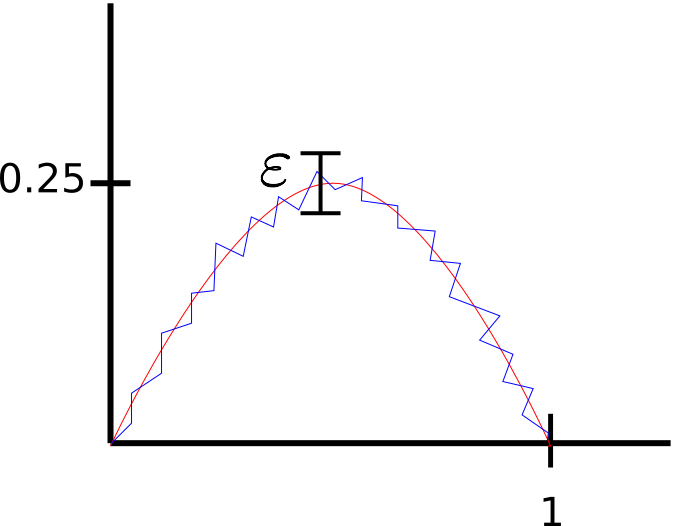
\includegraphics[width=0.5\textwidth]{Images/num2.png}
				\caption{The true solution \textcolor{blue}{$u_\varepsilon$} is a slightly perturbed version of \textcolor{red}{$x-x^2$}, perturbation is at most $\varepsilon$}
				\label{fig2}
			\end{figure}  
			\begin{figure}
				\centering
				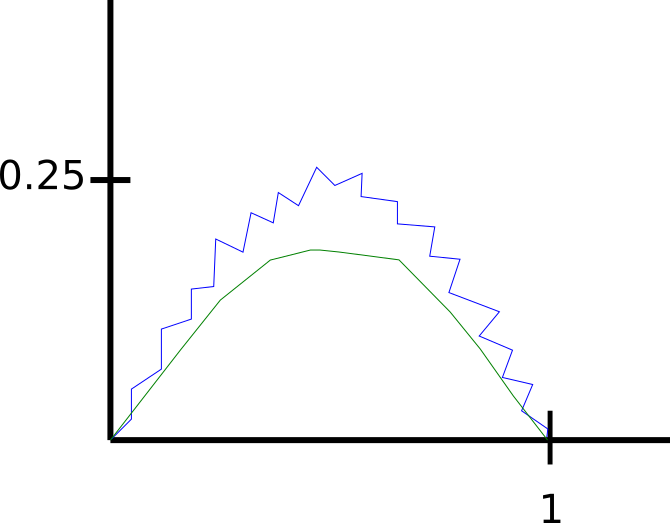
\includegraphics[width=0.5\textwidth]{Images/num3.png}
				\caption{For $h>\varepsilon$ the sequence of \textcolor{green}{FEM-solution}s converges to some other function than the \textcolor{blue}{true solution} of the problem}
				\label{fig3}
			\end{figure}